\subsection{Paraview}
\label{sec:paraview}

\subsubsection{Данные на одномерных сетках}
\label{sec:paraview-1d}

Заданные на сетке данные паравью показывает цветом.
Поэтому при загрузке одномерных сеток можно видеть картинку типа
\begin{center}
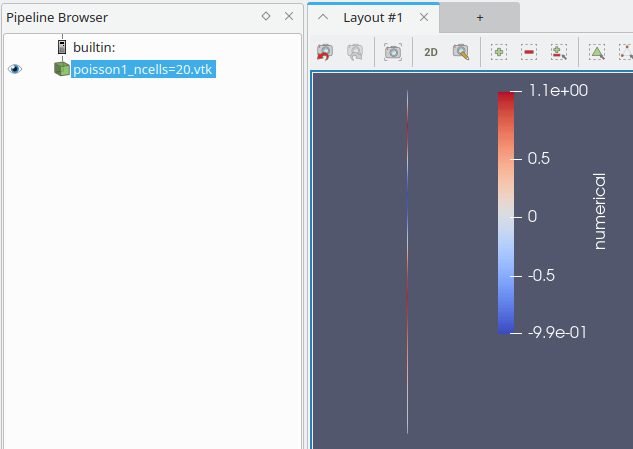
\includegraphics[width=0.5\linewidth]{howto_paraview_1d_1.png}
\end{center}
\paragraph{Развернуть изображение в плоскость xy}
\begin{center}
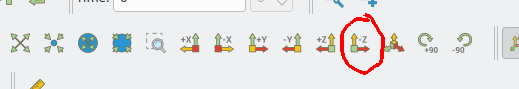
\includegraphics[width=0.5\linewidth]{howto_paraview_1d_2.png}
\end{center}
\paragraph{Отобразить данные в виде y-координаты} Для того, что бы данные отображались в качестве значения по оси ординат, к загруженному файлу необходимо
\begin{enumerate}
\item применить фильтр \ename{WarpByScalar} (В меню \ename{Filters->Alphabetical->Warp By Scalar})
\item в меню настройки фильтра указать поле данных, для отображения (numerical в примере ниже)
\item И настроить нормаль, вдоль которой будут проецироваться данные (в нашем случае ось y)
\end{enumerate}
\begin{center}
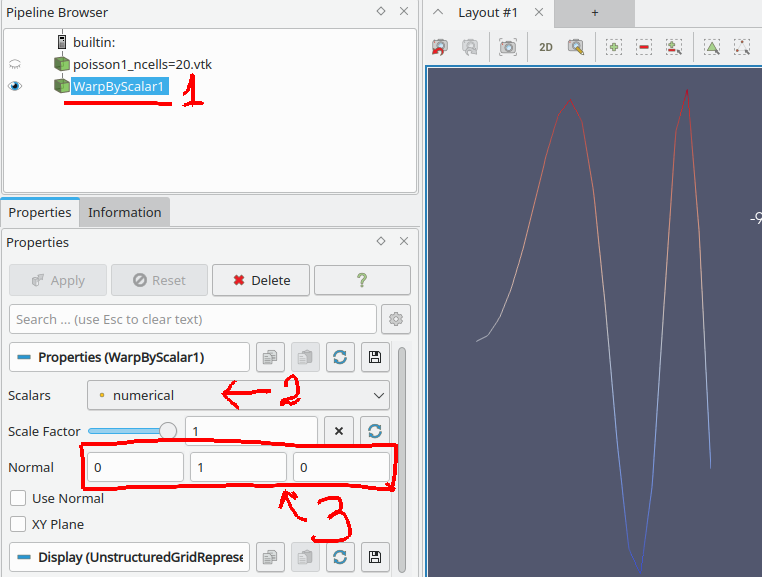
\includegraphics[width=0.5\linewidth]{howto_paraview_1d_3.png}
\end{center}

\paragraph{Цвет и толщина линии}
\begin{enumerate}
\item Включить подробные опции фильтра
\item Сменить стиль на \ename{Solid Color}
\item В меню \ename{Edit} выбрать желаемый цвет
\item В строке \ename{Line Width} указать толщину линии
\end{enumerate}
\begin{center}
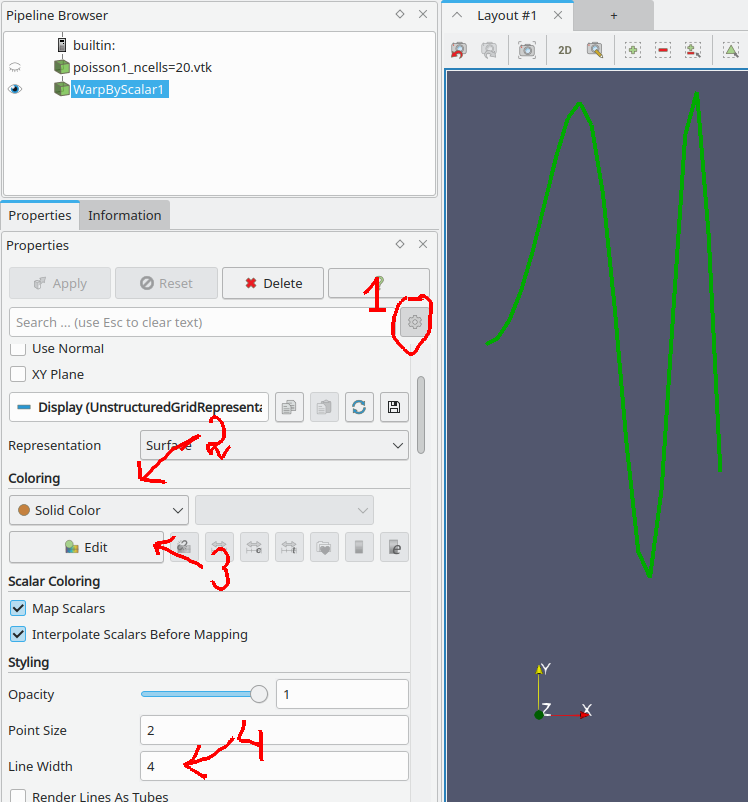
\includegraphics[width=0.6\linewidth]{howto_paraview_1d_4.png}
\end{center}

\paragraph{Настрока масштабов и отображение осей координат}
\begin{enumerate}
\item Отметье подробные настройки фильтра
\item В поле \ename{Transforming/Scale} Установите желаемые масштабы (в нашем случае растянуть в два раза по оси x)
\item Установите галку на отображение осей
\item откройте меню натройки осей
\item В нём включите подробные настроки
\item И также поставьте растяжение осей
\end{enumerate}
В случае, если масштабировать график не нужно, достаточно выполнить шаг 3.
\begin{center}
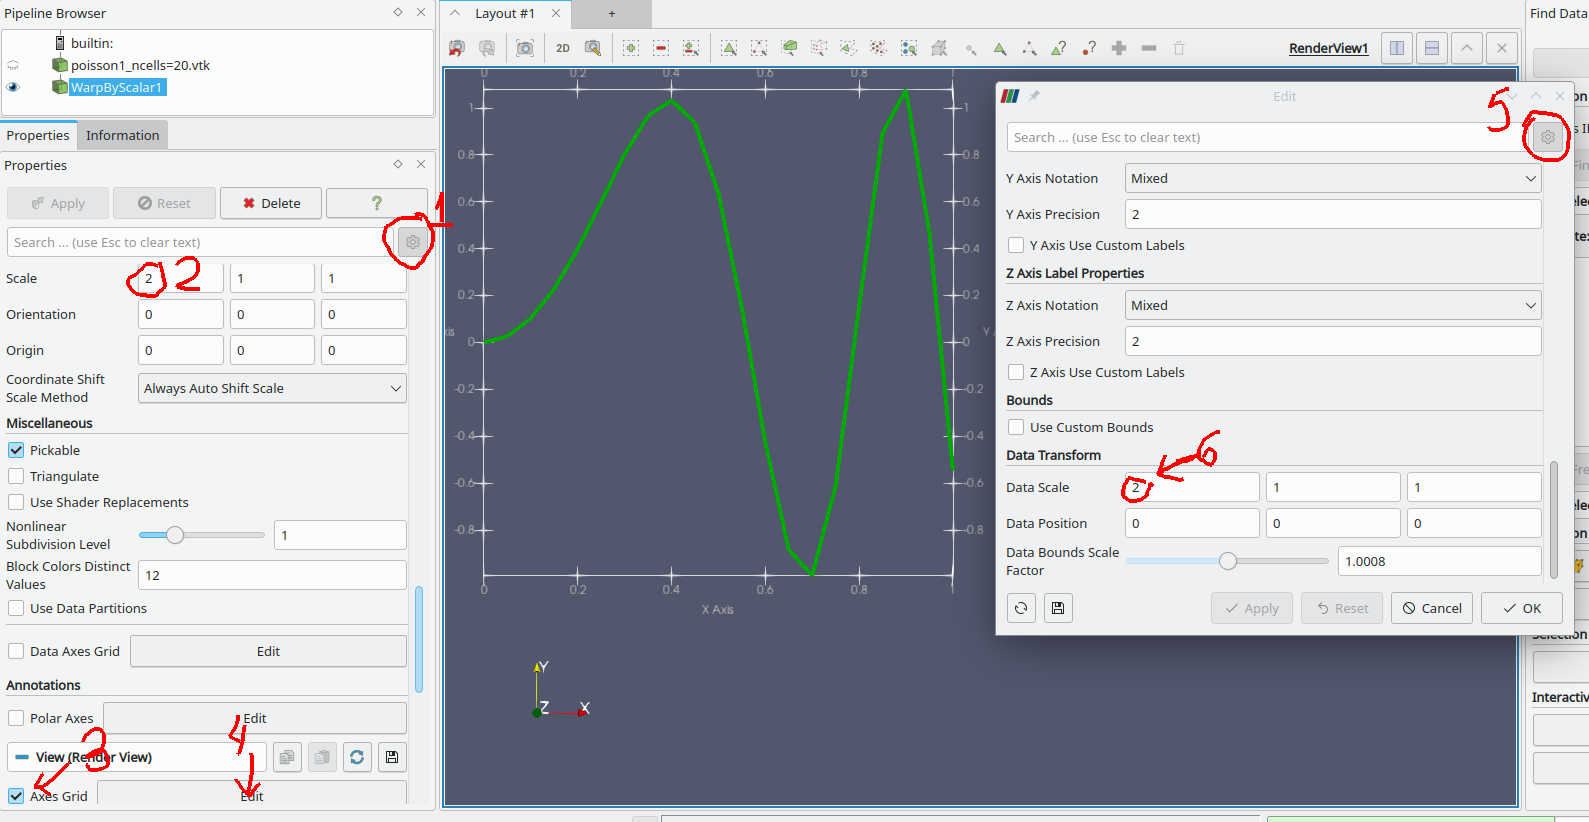
\includegraphics[width=0.9\linewidth]{howto_paraview_1d_5.png}
\end{center}

\paragraph{Построение графиков для нескольких данных}
Если требуется нарисовать рядом несколько графиков для разных данных из одного файла,
примените фильтр \ename{Warp By Scalar} для этого файла ещё раз, изменив поле \ename{Scalars} в настройке фильтра.
Для наглядности измените имя узла в Pipeline Browser на осмысленные
\begin{center}
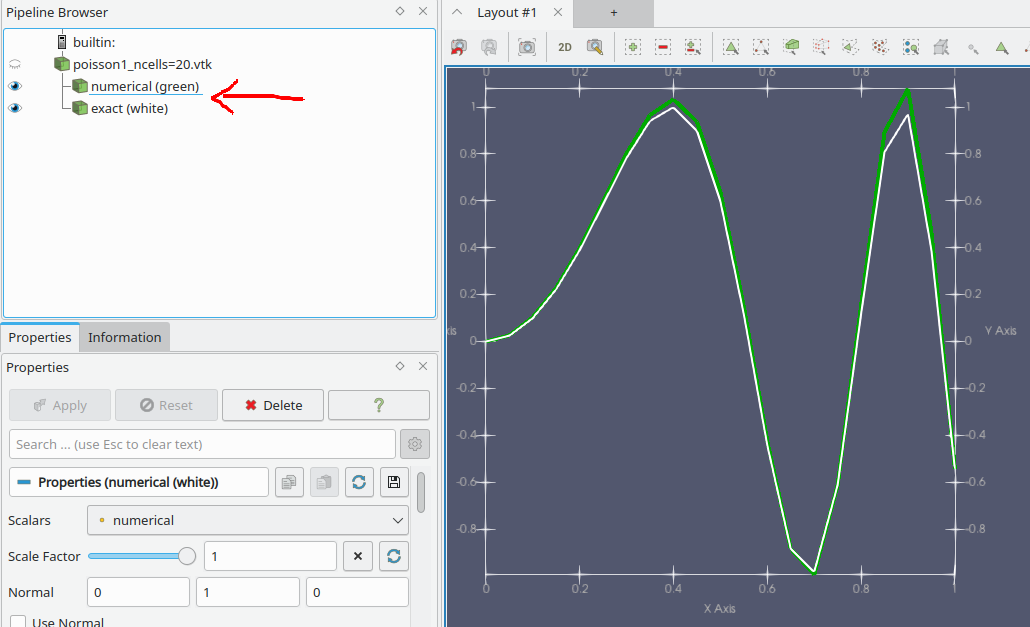
\includegraphics[width=0.8\linewidth]{howto_paraview_1d_6.png}
\end{center}

\paragraph{Обновление данных при изменении исходного файла}
В случае, если исходный файл был изменён, нужно в контекстном меню узла соответствующего файла
выбрать \ename{Reload Files} (или нажать F5). Если те же самые фильтры нужно применить для просмотра другого файла
нужно в этом меню нажать \ename{Change File}.
\begin{center}
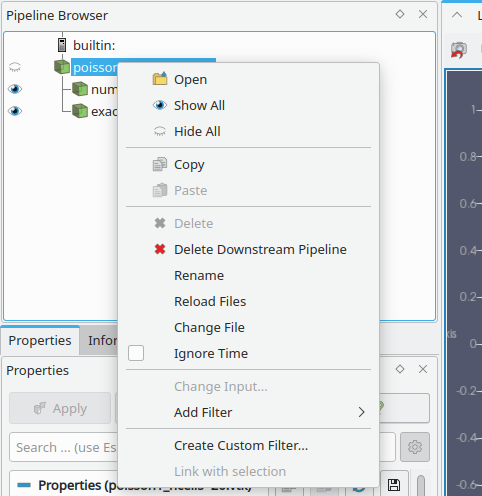
\includegraphics[width=0.4\linewidth]{howto_paraview_1d_7.png}
\end{center}

\subsubsection{Изолинии для двумерного поля}
\label{sec:paraview-isolines}

Ниже представлен алгоритм отрисовки изолиний для данных не сетке,
на которой решение изветно в узлах.
Если вы работаете с данными в ячейках (конечнообъёмная сетка),
следует предварительно применить фильтр \quo{Cell Data To Point Data}.

\begin{enumerate}
\item Нажмите иконку \ename{Contour} (или \ename{Filters/Contour})
      В настройках фильтра Contour by выберитее данные, по которым нужно строить изолинии.
\item В настройках фильтра удалите все существующие записи о значениях для изолиний
\item Добавьте равномерные значения. В появившемся меню установите необходимое количество изолиний и их диапазон.
\item Если необходимо, включите одновременное отображения цветного поля и изолиний.
\end{enumerate}

\begin{center}
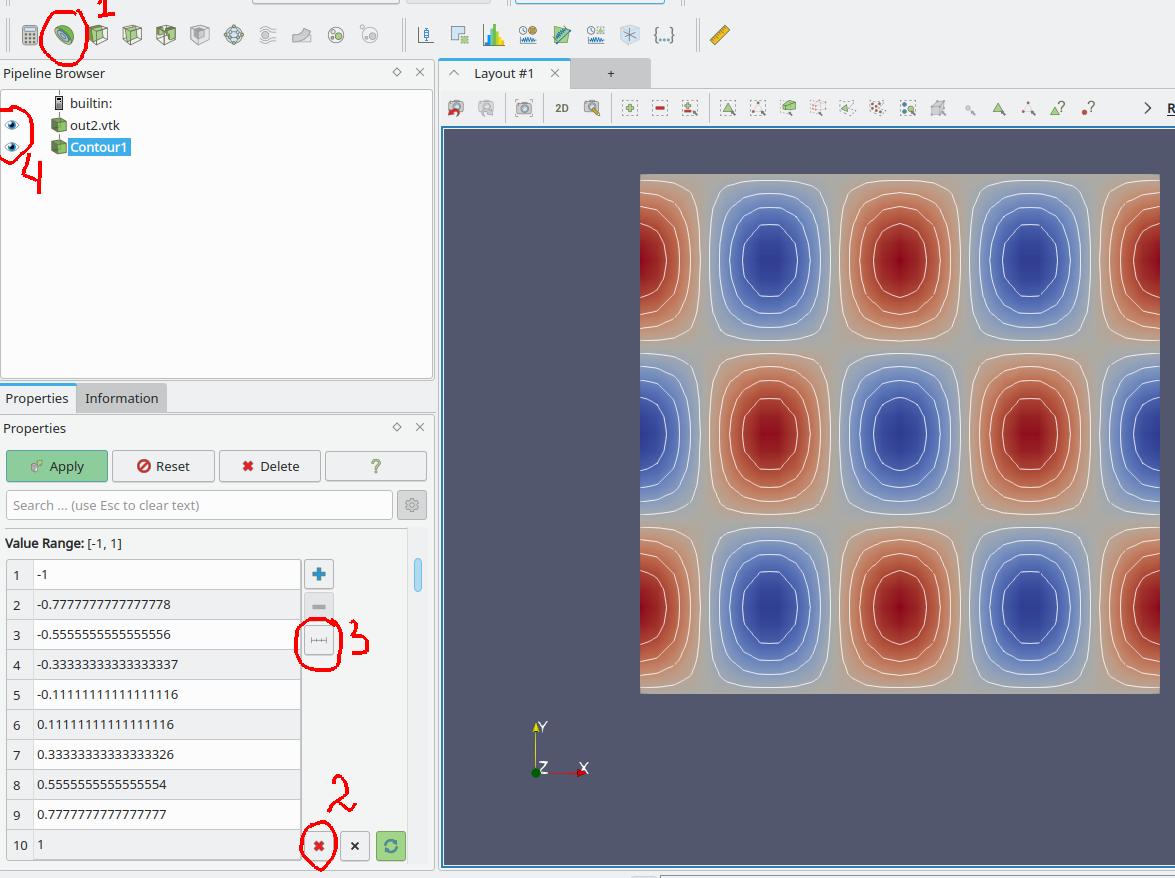
\includegraphics[width=0.7\linewidth]{howto_paraview_isolines_1.png}
\end{center}

\paragraph{Задание цвета и толщины изолинии}
В случае, если нужно сделать изолинии одного цвета, установите поле \ename{Coloring/Solid color} в 
настройках фильтра. Там же в меню \ename{Edit} можно выбрать цвет.
Для установления толщины линии включите подробные настройки и найдите там опцию \ename{Styling/Line Width}.
\begin{center}
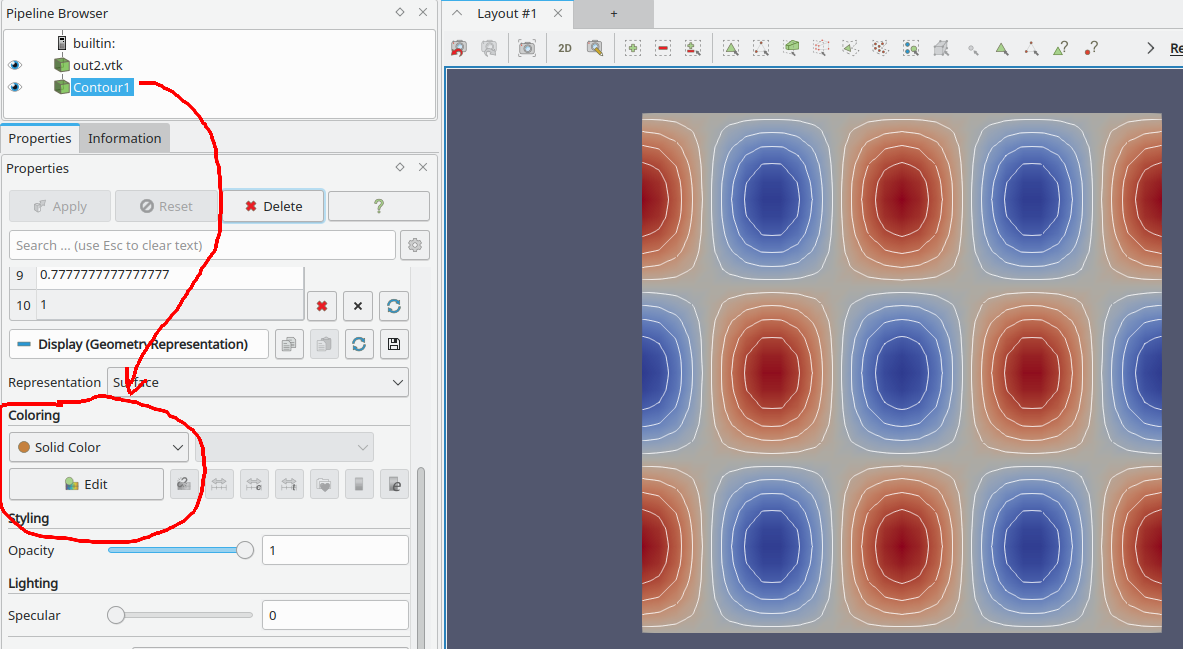
\includegraphics[width=0.7\linewidth]{howto_paraview_isolines_2.png}
\end{center}

\subsubsection{Данные на двумерных сетках в виде поверхности}
\label{sec:paraview-2d}

По аналогии с  одномерным графиком (п.~\ref{sec:paraview-1d}), двумерные поля так же
можно отобразить, проектируя данные на геометрическую координату для получения
объёмного графика. Для этого
\begin{enumerate}
\item Включите фильтр \ename{Filters/Warp By Scalar}
\item В настройках фильтра установите данные, которые будут проектироваться на координату z
\item Установите нормаль для проецирования (ось z)
\item Если нужно, выберите масштабирования для этой координаты
\item После нажатия \ename{Apply} включите трёхмерное отображение
\item Если данные не видно, обновите экран.
\end{enumerate}
\begin{center}
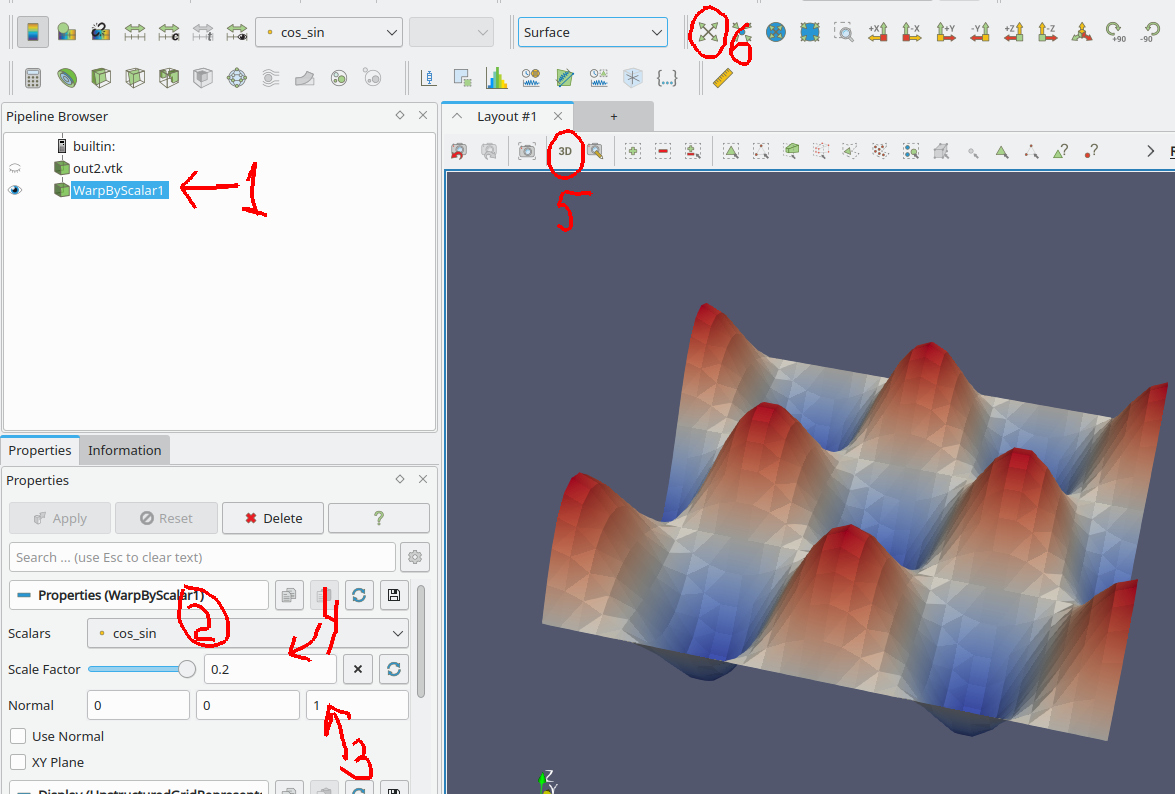
\includegraphics[width=0.9\linewidth]{howto_paraview_2d_as_3d.png}
\end{center}

\subsubsection{Числовых значения в точках и ячейках}
\label{sec:paraview-show-data}

Иногда в процессе отладки или анализа результатов расчёта
требуется знать точное значение поля в заданном узле или ячейке сетки.
Для этого

\begin{enumerate}
\item Включить режим выделения точек или ячеек (иконка (1 на рисунке) или горячие клавиши \ename{s}, \ename{d}).
      Выделить мышкой интересующую область
\item В окне \ename{Find data} (или \ename{Selection Inspector} для старых версий Paraview) отметить поле, которое должно отображаться 
      в центрах ячеек и в точках (2 на рисунке). Если такого окна нет, включить его из основного меню \ename{View}.
\end{enumerate}

\begin{center}
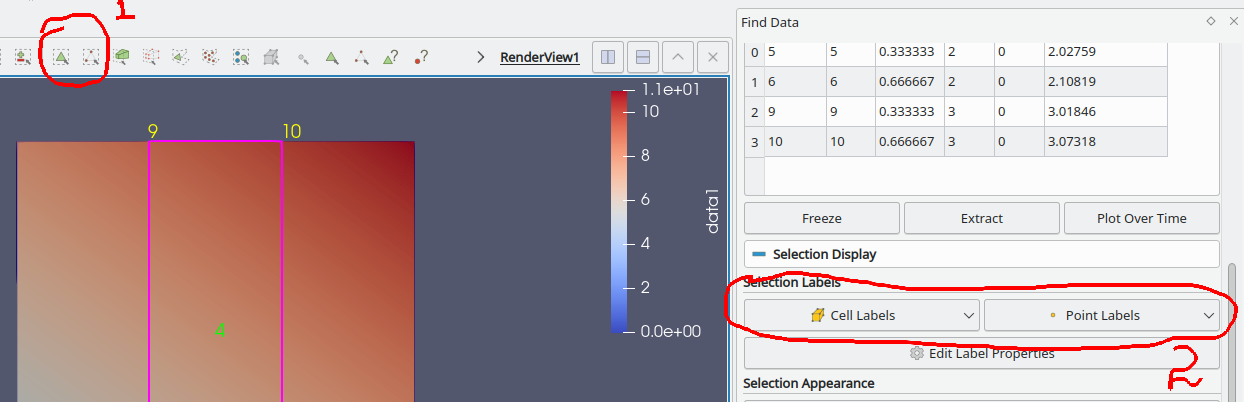
\includegraphics[width=0.8\linewidth]{howto_paraview_show_labels.png}
\end{center}

\subsubsection{Векторные поля}
\label{sec:paraview-glyph}

Открыть файл vtk или vtk.series, который содержит
векторное поле. Далее
\begin{enumerate}
\item Создать фильтр \ename{Glyph}
\item Задать двумерный тип стрелки
\item Сместить центр стрелки, чтобы она исходила из точки, к которой приписана
\item Отметить необходимое векторное поле в качестве ориентации
\item Отметить необходимое векторное поле для масштабирования
      Нажать \ename{Apply}.
\end{enumerate}

\begin{center}
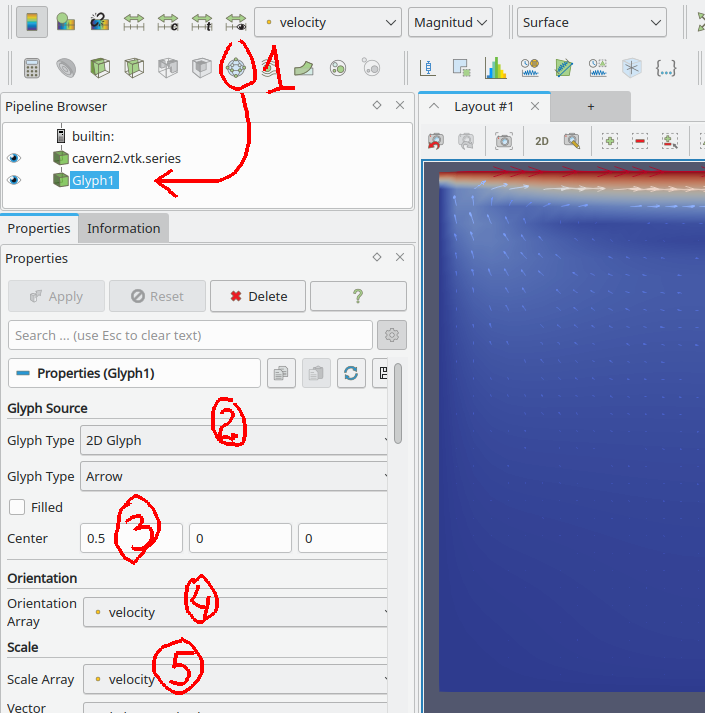
\includegraphics[width=0.6\linewidth]{glyph-1.png}
\end{center}

\paragraph{Настройка отображения стрелок}
\begin{enumerate}
\item Выбрать необходимый \ename{Glyph-mode}. Если сетка небольшая, то можно \ename{All Points}.
\item Установить белый цвет для стрелок. Нажать Apply.
\end{enumerate}

\begin{center}
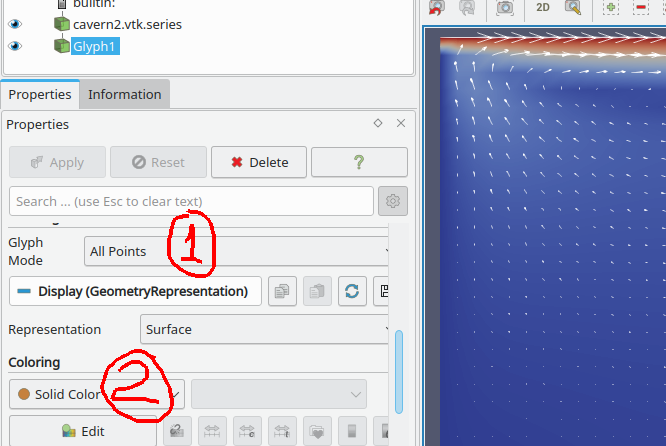
\includegraphics[width=0.4\linewidth]{glyph-2.png}
\end{center}

\paragraph{Уменьшения разброса по длине стрелок}
Если разброс по длинам стрелок слишком велик, его можно подравнять,
введя новую функцию $|\vec v|^{\alpha}$ -- длина вектора в степени меньше единицы (например, $\alpha=0.7$).
Такую функцию можно создать через калькулятор

\begin{enumerate}
\item Начиная от загруженного файла создать фильтр \ename{Calculator}
\item Там вбить необходимую формулу
\end{enumerate}
\begin{center}
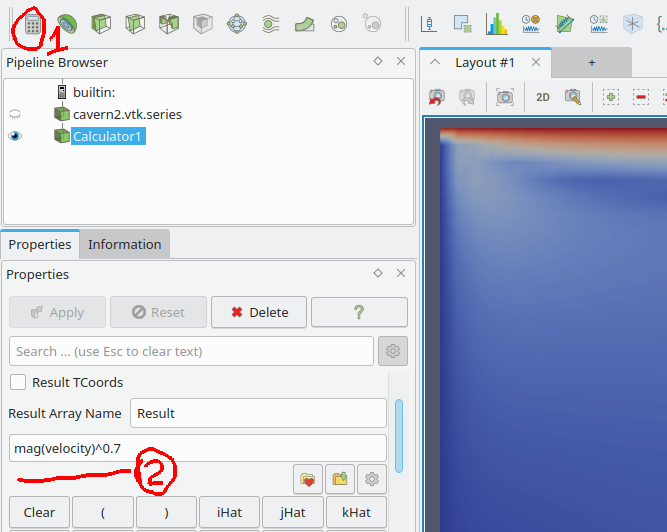
\includegraphics[width=0.6\linewidth]{glyph-3.png}
\end{center}
Созданную функцию нужно прокинуть в \ename{Glyph} в качестве коэффициента масштабирования
\begin{enumerate}
\item В \ename{Scale Array} фильтра \ename{Glyph} указать уже результат работы \ename{Calculator}-a (\ename{Result} по умолчанию),
\item Подтянуть значение \ename{Scale Factor} до приемлимого
\item Не забыть отключить вспомогательное поле \ename{Calculator} из отображения
\end{enumerate}
\begin{center}
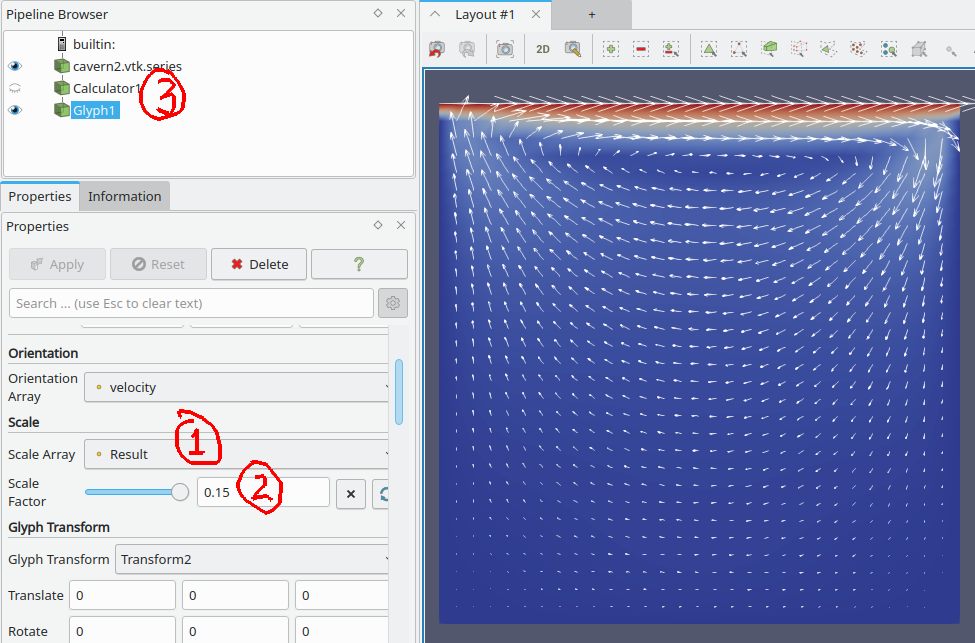
\includegraphics[width=0.6\linewidth]{glyph-4.png}
\end{center}

\subsubsection{Значение функции вдоль линии}
\label{sec:paraview-plot-over-line}

\begin{enumerate}
\item
Выбрать фильтр \ename{Plot Over Line} иконкой или в меню \ename{Filters}
\item
Установить начальную и конечную точку сечения
\item
Можно использовать привязку к узлам сетки с помощью горячих клавиш (в подсказках написано)
\item
Можно установить координаты руками в соответствующем поле. Для двумерных задач проследить,
что координата Z равна нулю
\item
Нажать \ename{Apply}
\end{enumerate}

\begin{center}
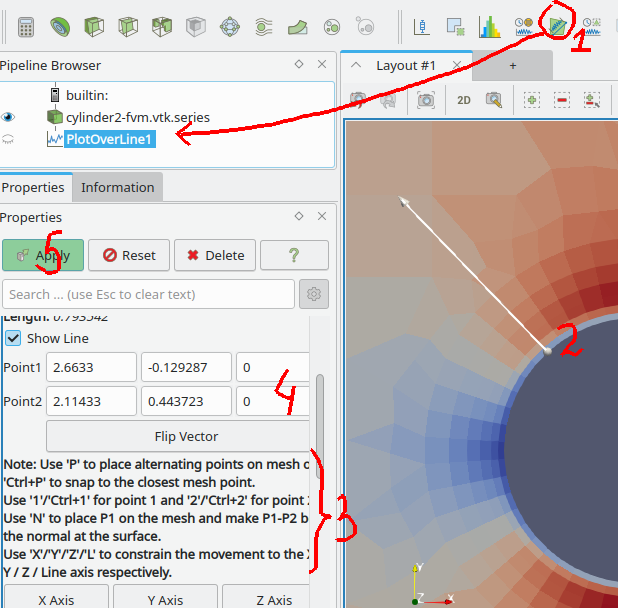
\includegraphics[width=0.4\linewidth]{howto_paraview_plot_over_line_1.png}
\end{center}

\paragraph{Настройка графика}
\begin{enumerate}
\item
После установок появится дополнительное окно типа \ename{Line Chart View} с нарисованным графиком.
\item
Сделав это окно активным в настройках фильтра \ename{PlotOverLine}
можно выбрать, какие поля рисовать (\ename{Series Parameters})
\end{enumerate}

\begin{center}
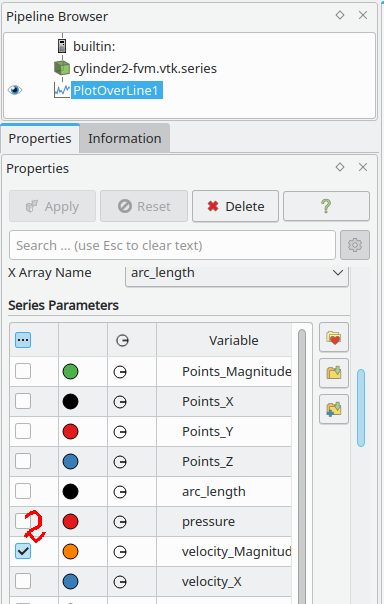
\includegraphics[width=0.2\linewidth]{howto_paraview_plot_over_line_3.png}
\quad
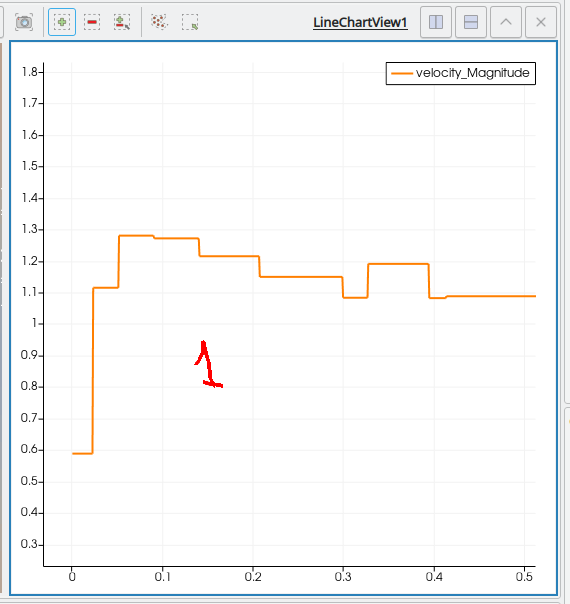
\includegraphics[width=0.3\linewidth]{howto_paraview_plot_over_line_2.png}
\end{center}

\paragraph{Отрисовка в отдельном окне}
\begin{enumerate}
\item
Открыть новую вкладку
\item
Выбрать \ename{Line Chart View}
\item
Выбрать предварительно созданный фильтр с одномерным графиком
\end{enumerate}
\begin{center}
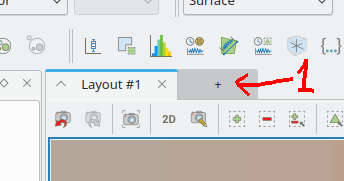
\includegraphics[width=0.2\linewidth]{howto_paraview_plot_over_line_4.png}
\quad
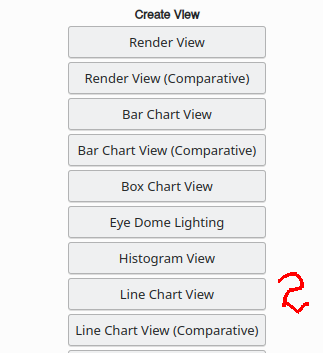
\includegraphics[width=0.3\linewidth]{howto_paraview_plot_over_line_5.png}
\quad
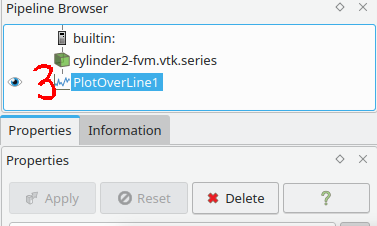
\includegraphics[width=0.3\linewidth]{howto_paraview_plot_over_line_6.png}
\end{center}
